\subsection{自更新盲密钥管理}
\label{subsec:sgxdedup-key-management}

每个客户端都通过一个共享的盲密钥与密钥安全区安全通信,以防止密钥服务器 (\S\ref{subsec:sgxdedup-arch})窃听。为了产生盲密钥,一种直接的方法是直接在密钥安全区和每个客户端之间实现密钥协商协议。但是,密钥安全区需要即时验证客户端访问权限(例如,客户端可以更新或撤销其云存储服务订阅)。这种动态认证给密钥安全区带来了性能负担。

\begin{figure}[!htb]
\centering
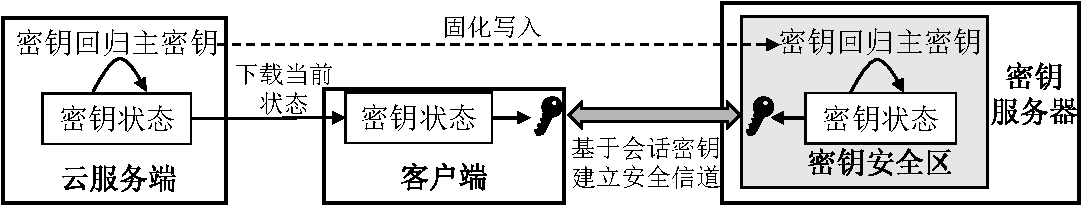
\includegraphics[width=\textwidth]{pic/sgxdedup/keyRegression.pdf}
\caption{可更新的盲密钥管理:云服务端和密钥安全区可以根据其盲密钥状态导出新的盲密钥,而客户端只能从云服务端下载当前密钥状态,并产生最新的盲密钥}
\label{fig:sgxdedup-keymanage}
\end{figure}

如图~\ref{fig:sgxdedup-keymanage}所示,\sysnameS 在云服务端的帮助下管理盲密钥。在系统初始化期间,云服务端将一个盲秘密种子$\kappa$硬编码到密钥安全区代码中。每个客户端从云服务端下载一个\textit{密钥状态(key state)}(源自于$\kappa$;见下文),并基于该密钥状态生成对应的盲密钥,用于与密钥安全区的安全通信。本文如此设计的考虑有以下三点:
\begin{itemize}
    \item 首先,当客户端对云服务端发出任何上传/下载请求时,云服务端可以检查客户端是否被授权。
    \item 其次,本文可以从$\kappa$派生(而不是直接使用$\kappa$)一系列可更新的盲密钥,以防止被撤销/被攻击的客户端持续访问密钥安全区。
    \item 可更新密钥管理定期更新盲密钥,要求客户端定期在云服务端进行验证,可以防止在线暴力攻击(\S\ref{subsec:background-encrypted-deduplication-key}),而不会主动降低密钥生成速率\cite{bellare2013DupLESS}。
\end{itemize}

\sysnameS 基于密钥回归(\textit{key regression})\cite{fu06}导出可更新的盲密钥,同时确保每个客户端和密钥安全区中的盲密钥是一致的。具体来说,密钥回归使用一系列密钥状态$S[1]、S[2]、\ldots、S[m]$,每个密钥状态都可用于派生密钥(例如,通过哈希函数)。它允许密钥安全区和云服务端执行密钥状态更新(\textit{rekeying})以使用盲秘密种子从旧密钥状态派生新密钥状态(例如,从$S[1]$导出$S[2]$),使得客户端无法在不知道盲秘密种子的情况下获得有关新密钥状态的任何信息。同时,它允许每个客户端从新密钥状态派生任何旧密钥状态(例如,从$S[2]$派生$S[1]$)。

为了在\sysnameS 中实现密钥回归,本文使用$\kappa$作为在云服务端和密钥安全区之间共享的盲秘密种子,用于派生新的密钥状态和盲密钥。在每次上传开始前,客户端首先从云服务端下载最新的密钥状态$S[i]$,并向密钥服务器查询密钥安全区接受的盲密钥的版本号$j$。鉴于密钥安全区可能无法及时更新盲密钥(例如,在计划的更新密钥时间内正在提供密钥生成服务),$j$通常小于$i$(即$S[j]$在$S[i]$之前)。然后客户端从$S[i]$派生出$S[j]$并导出对应的盲密钥$K[j]$,最终基于相同的$K[j]$与密钥安全区通信。请注意,云服务端可以导出$K[j]$,但它无法窃听每个客户端和密钥安全区之间的通信,因为通过客户端和密钥服务器之间的通信受到SSL/TLS协议的额外保护(参见本文在\S\ref{subsec:sgxdedup-threat} 中提出的安全假设)。

\sysnameS 在云服务端和密钥服务器中实现了同步计时器,在周期性的时间间隔内自动触发盲密钥更新。这里,密钥服务器发出\textit{Rekeying ECall}以在达到预定的密钥更新时间且密钥服务器结束对已连接客户端的服务时通过安全区内部调用触发安全区内盲密钥更新。

本文实现了基于哈希的密钥回归方案\cite{fu06}以获得较高的密钥更新性能。具体来说,本文定义了参数$n$(默认设置为$2^{20}$\cite{fu06})来指示可进行的最大密钥更新次数。 云服务端和密钥安全区计算第$i$个密钥状态为$S[i] = {\bf H}^{n-i+1}(\kappa)$,每个客户端派生相应的盲密钥为$K[i] = {\bf H}(S[i] || 0^8)$,其中${\bf H}^{n-i+1}()$迭代调用安全哈希函数${\bf H}()$共计$n-i+1$次,$||$是连接运算符。若客户端需要导出旧密钥$K[j]$,则客户端下载$S[i]$并计算$S[i-1] = {\bf H}(S[i])$直到得到目标密钥状态$S[j]$,进而导出盲密钥$K[j] = {\bf H}(S[j] || 0^8)$。
